\documentclass{article}
\usepackage{amsmath}
\usepackage{amssymb}
\usepackage[usenames, dvipsnames]{color}
\usepackage{gensymb}
\usepackage{hyperref}
\usepackage{tikz}
\usepackage{geometry}
\usepackage[normalem]{ulem}

\title{\vspace{-3em}The Sky-Diving Trainhopper\vspace{-3em}}

\geometry{letterpaper, portrait, margin=0.5in}

\definecolor{myred1}{RGB}{255, 0, 0}
\definecolor{myyellow1}{RGB}{255, 255, 219}
\definecolor{mygreen1}{RGB}{0, 255, 0}
\definecolor{mygreen2}{RGB}{0, 126, 0}
\definecolor{myblue1}{RGB}{0, 0, 255}

\begin{document}

\fontsize{14}{16}\selectfont

% center the title
\maketitle

Om is a skydiving trainhopper. A freighter steam locomotive is going downhill on a straight track that makes an angle of elevation with the ground of $\theta=37.13\degree$. Unfortunately, the train's engine has failed and the wheels are sliding down the frictionless tracks. Luckily, the train has a backup jet propulsion engine. The horizontal distance the hill comprises is 300 meters. Om is attempting to skydive onto the train. The train has a mass of $m=550000$ kg.

\section{How fast is Om dying?} 
Om falls from 500 meters above and 300 meters from the mountain, which rises at an incline of 37.13\degree. The force of gravity on Om is 620N. \textbf{Solve for the amount of time it takes for Om to reach the base of the mountain.} \\
(5 points)

\section{How fast is that engine going?}
Use the time $t$ you found from the previous problem. \textbf{Solve for the work that the jet propulsion engine needs to do on the train for it to reach the bottom of the hill just in time to catch Om at the front of the engine.} \\
(4 points)

\section{How much faster does the train go after Om dies?}
Find the increased velocity of the freighter after Om dies on the train. 

\pagebreak

\section{Solutions}

For each section half credit is awarded for solutions that use correct methods, with the other half being awarded to solving the section accurately using the given figures.

\subsection{How fast is Om dying?}
\begin{enumerate}
    \item Find Om's mass. (1 point)\\
    \(F = ma\)
    \(m =\frac{F}{a}\)
    \(\frac{620N}{9.8}=63.26kg\)

    \item Find the height of Om above the Earth. (1 point) \\
    
    \(90-37.13\degree = 52.87\degree\) \\
    \(300m \cdot \tan 52.87\degree = 396.24m\) \\
    \(396.24m + 500m = 896.24m\)

    \item Find the final velocity of Om. (2 points) \\

    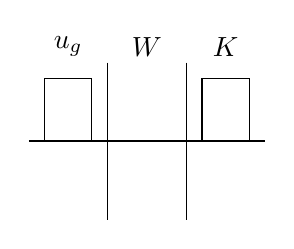
\begin{tikzpicture}
    \draw [thick] (0,0) -- (3,0);
    \draw (1,1) -- (1,-1);
    \draw (2,1) -- (2,-1);
    \draw (0.5,1.2) node {$u_g$};
    \draw (1.5,1.2) node {$W$};
    \draw (2.5,1.2) node {$K$};
    \draw[rectangle, draw=black] (0.2,0) rectangle (0.8,0.8);
    \draw[rectangle, draw=black] (1.2,0) rectangle (1.8,0.0);
    \draw[rectangle, draw=black] (2.2,0) rectangle (2.8,0.8);
    \end{tikzpicture}

    \(mgh = \frac{1}{2}mv^2\) \\
    \(63.26(9.8)(896.24) = \frac{1}{2}63.26v^2\) \\
    \(555622.20 = 31.63v^2\) \\
    \(17566.30 = v^2\) \\
    \(132.54\frac{m}{s}^2 = v\)

    \item Find the time it takes Om to reach the base of the mountain. (1 point) \\\
    \(t = \frac{d}{v}\) \\
    \(t = \frac{896.24}{132.54}\) \\
    \(t = 6.76s\)
\end{enumerate}

\subsection{How fast is that engine going?}

\begin{enumerate}
    \item Find the distance the train is going. (1 point)

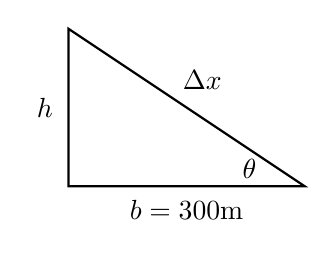
\begin{tikzpicture}
    \draw [thick] (0,0) -- (3,0) -- (0,2) -- cycle;
    \draw (1.5,-0.3) node {$b=300$m};
    \draw (-0.3,1) node {$h$};
    \draw (1.7,1.35) node {$\Delta x$};
    \draw (2.3,0.22) node {$\theta$};
\end{tikzpicture}

\begin{align*}
    h=b\tan\theta 
    \Longrightarrow h=(300\text{m})\tan(37.13\degree) \approx 227.135\text{m}
    \\
    \Delta x=b\sec\theta
    \Longrightarrow \Delta x=(300\text{m})\sec(37.13\degree) \approx 376.285\text{m}
\end{align*}

\item Find the impulse at which the train moves. (3 points)

System: train and Earth
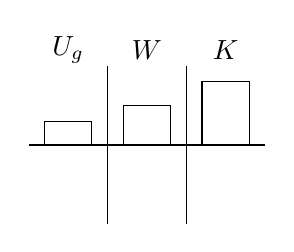
\begin{tikzpicture}
    \draw [thick] (0,0) -- (3,0);
    \draw (1,1) -- (1,-1);
    \draw (2,1) -- (2,-1);
    \draw (0.5,1.2) node {$U_g$};
    \draw (1.5,1.2) node {$W$};
    \draw (2.5,1.2) node {$K$};
    \draw[rectangle, draw=black] (0.2,0) rectangle (0.8,0.3);
    \draw[rectangle, draw=black] (1.2,0) rectangle (1.8,0.5);
    \draw[rectangle, draw=black] (2.2,0) rectangle (2.8,0.8);
\end{tikzpicture}

\begin{align*}
    u_k=\frac{1}{2}mv^2 \quad u_g=mgh \\
    \Longrightarrow W=\frac{1}{2}mv^2-mgh \\
    v_f=v_0+at 
    \quad x_f=x_0+v_0t+at^2 \Longrightarrow x_f=\frac{1}{2}at^2 \Longrightarrow \frac{2x_f}{t}=at \\
    v_f=\frac{2x_f}{t} \\
    \Longrightarrow W=m(\frac{1}{2}\biggr(\frac{2x_f}{t}\biggr)^2-gh) \\
    \Longrightarrow W=m(2\biggr(\frac{x_f}{t}\biggr)^2-gh)
    \Longrightarrow W=(550000\text{kg})(2\biggr(\frac{376.285\text{m}}{6.76\text{s}}\biggr)^2-\biggr(9.8\frac{\text{m}}{\text{s}^2}\biggr)(227.135\text{m})) \\
    \Longrightarrow 2184004499 \text{J}
\end{align*}

\end{enumerate}

\subsection{How much faster does the train go after Om dies?}
System: Om and train \\
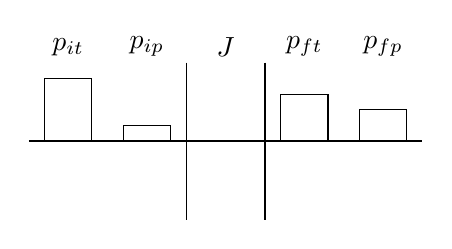
\begin{tikzpicture}
    \draw [thick] (0,0) -- (5,0);
    \draw (2,1) -- (2,-1);
    \draw (3,1) -- (3,-1);
    \draw (0.5,1.2) node {$p_{it}$};
    \draw (1.5,1.2) node {$p_{ip}$};
    \draw (2.5,1.2) node {$J$};
    \draw (3.5,1.2) node {$p_{ft}$};
    \draw (4.5,1.2) node {$p_{fp}$};
    \draw[rectangle, draw=black] (0.2,0) rectangle (0.8,0.8);
    \draw[rectangle, draw=black] (1.2,0) rectangle (1.8,0.2);
    \draw[rectangle, draw=black] (3.2,0) rectangle (3.8,0.6);
    \draw[rectangle, draw=black] (4.2,0) rectangle (4.8,0.4);
\end{tikzpicture}

\begin{align*}
    p_{ip}=m(v_0+at)
    \Longrightarrow p_{ip}=(63.26\text{kg}) \biggr(9.8\frac{\text{m}}{\text{s}^2}\biggr) \cdot 6.76\text{s} 
    \approx 4190.848 \frac{\text{kg} \cdot \text{m}}{\text{s}}\\
    p_{it}=2m\frac{\Delta x{t}}
    \Longrightarrow p_{it}=2(550000\text{kg})\cdot \frac{376.285\text{m}}{6.76\text{s}}
    \approx 61229811.35 \frac{\text{kg} \cdot \text{m}}{\text{s}} \\
    p_{it}+p_{ip}+\Delta p=p_{ft}+p_{fp} 
    \Longrightarrow p_{it}+p_{ip}=v_f(m_t+m_p)
    \Longrightarrow v_f=\frac{p_{it}+p_{ip}}{m_t+m_p} \\
    v_f=\frac{4190.858 \frac{\text{kg} \cdot \text{m}}{\text{s}}+61229811.35 \frac{\text{kg} \cdot \text{m}}{\text{s}}}{63.26 \text{kg} + 550000 \text{kg}} 
    = 111.32 \frac{\text{m}}{\text{s}}
\end{align*}
\end{document}
